\chapter{消化与吸收}\label{ch:b1:digestion-absorption}

奶牛每天吃 10 千克草，靠乙酸为生；马吃同样的草，
部分靠葡萄糖为生；兔子吃自己夜里排出的粪便，没有这些粪便就会生病。
三者自身都不能\omterm{def:b1:digestion-absorption:nutrition}{消化}\omterm{def:b1:carbohydrates:polysaccharide}{纤维素}，却都借助体内能分解\omterm{def:b1:carbohydrates:polysaccharide}{纤维素}的细菌完成\omterm{def:b1:digestion-absorption:nutrition}{消化}。
人类自身不能做到这一点，但一顿面包、肉和黄油，
几小时内就能\omterm{def:b1:digestion-absorption:nutrition}{消化}为\omterm{def:b1:carbohydrates:monosaccharide}{糖类}、\omterm{def:b1:proteins:aminoacid}{氨基酸}和\omterm{def:b1:lipids:fattyacid}{脂肪酸}，
同时每天经过一层\omterm{def:b1:cell-unit-of-life:cell}{细胞}厚的肠壁\omterm{def:b1:digestion-absorption:nutrition}{吸收} 9 升水。
本章介绍哺乳动物的\omterm{prop:b1:digestion-absorption:tract}{消化道}，
分解食物的酶和分泌物，摄取这些碎片的\omterm{def:b1:cell-unit-of-life:cell}{细胞}，
调控整个过程节奏的信号，
以及植食性动物与微生物的共生关系，
使其能够利用哺乳动物自身的酶无法分解的食物。

\section{异养营养}

\begin{definition}[营养、消化与吸收]\label{def:b1:digestion-absorption:nutrition}
\index{消化}\index{吸收}
\omterm{def:b1:organism-environment:trophy}{异养}生物必须从食物中获取能量和碳、
以及它自身不能合成的\omterm{def:b1:proteins:aminoacid}{氨基酸}和\omterm{def:b1:lipids:fattyacid}{脂肪酸}（\cref{ch:b1:biosyntheses-integration}）、
维生素、无机盐和水。食物以大分子形式进入——\omterm{def:b1:carbohydrates:polysaccharide}{淀粉}、
\omterm{def:b1:proteins:peptide}{蛋白质}、\omterm{def:b1:lipids:triglyceride}{脂肪}——它们不能穿过膜。\emph{消化}是
酶对其进行水解，使之成为足够小、能被吸收的单体：
葡萄糖、\omterm{def:b1:proteins:aminoacid}{氨基酸}、\omterm{def:b1:lipids:fattyacid}{脂肪酸}和甘油、\omterm{def:b1:nucleic-acids:nucleotide}{核苷酸}。
\emph{吸收}是这些单体穿过肠道\omterm{def:b1:body-plans-tissues:epithelium}{上皮}、
进入血液或\omterm{def:b1:mammal-organization:compartments}{淋巴液}的过程。在动物体内，消化是\emph{\omterm{def:b1:cell-unit-of-life:cell}{细胞}外}的，
发生在两端开口的管腔中，
这使食物能随着移动分阶段加工，
也使管道各区段分工明确。
\end{definition}

\begin{proposition}[哺乳动物的消化道]\label{prop:b1:digestion-absorption:tract}
\index{消化道}
哺乳动物的\omterm{prop:b1:digestion-absorption:tract}{消化道}从口到肛门分为若干区段，
每段都有各自的\omterm{def:b1:body-plans-tissues:epithelium}{上皮}、分泌物和肌肉：
\emph{口腔}，牙齿在此咀嚼，唾液湿润食物并开始\omterm{def:b1:digestion-absorption:nutrition}{消化}\omterm{def:b1:carbohydrates:polysaccharide}{淀粉}；
\emph{食管}，仅是一条管道；
\emph{胃}，一个含酸的囊，\omterm{def:b1:proteins:peptide}{蛋白质}在此被解折叠并切断，
食物在此暂存，并以糊状的食糜排出；
\emph{小肠}——十二指肠、空肠、回肠，人体中长约 6 米——是
\emph{肝脏}（胆汁）与\emph{胰腺}（酶和碳酸氢盐）分泌物的汇入之处，
\omterm{def:b1:digestion-absorption:nutrition}{消化}在此完成，几乎全部\omterm{def:b1:digestion-absorption:nutrition}{吸收}也在此进行；
\emph{大肠}，在此回收水分，
密集的微生物群落\omterm{def:b1:respiration-fermentation:fermentation}{发酵}残余物质；以及直肠。
管壁中的肌肉（\cref{ch:b1:body-plans-tissues}）混合内容物，
并通过\emph{蠕动}推动其前进；括约肌在各阶段将内容物暂留。
\end{proposition}

\begin{omfigure}
\begin{tikzpicture}[font=\footnotesize, >=Stealth, line cap=round,
  reg/.style={draw, thick, rounded corners=4pt, minimum height=9mm, text width=24mm, align=center, fill=white}]
  \node[reg, fill=omDef!12] (m) at (0,0) {\textbf{口腔}\\ pH 7};
  \node[reg, fill=omThm!12] (st) at (3.2,0) {\textbf{胃}\\ pH 2};
  \node[reg, fill=omProp!12] (si) at (6.4,0) {\textbf{小肠}\\ pH 7--8};
  \node[reg, fill=omExo!12] (li) at (9.6,0) {\textbf{大肠}\\ pH 6--7};
  \draw[->, very thick] (m) -- (st); \draw[->, very thick] (st) -- (si); \draw[->, very thick] (si) -- (li);
  \node[anchor=north, align=center, text width=28mm] at (0,-0.6) {咀嚼；唾液淀粉酶作用于淀粉};
  \node[anchor=north, align=center, text width=28mm] at (3.2,-0.6) {HCl、胃蛋白酶作用于蛋白质；黏液；储存、混合};
  \node[anchor=north, align=center, text width=30mm] at (6.4,-0.6) {胆汁、胰酶、刷状缘酶；几乎所有物质的吸收};
  \node[anchor=north, align=center, text width=28mm] at (9.6,-0.6) {回收水分和盐；微生物发酵；粪便};
  \node[draw, thick, rounded corners=3pt, fill=omProp!25, inner sep=3pt, align=center] (liv) at (4.8,1.7) {肝脏：胆汁};
  \node[draw, thick, rounded corners=3pt, fill=omProp!25, inner sep=3pt, align=center] (pan) at (8.0,1.7) {胰腺：酶，\\ 碳酸氢盐};
  \draw[->, thick, omProp!80!black] (liv) -- (5.9,0.5); \draw[->, thick, omProp!80!black] (pan) -- (6.9,0.5);
  \node[anchor=west, font=\scriptsize, gray] at (10.9,0) {通过时间：\qtyrange{24}{48}{h}};
\end{tikzpicture}

{\small 哺乳动物\omterm{prop:b1:digestion-absorption:tract}{消化道}各区段及其功能。
位于\omterm{def:b1:digestion-absorption:nutrition}{消化}管外的两个腺体，肝脏和胰腺，将其
分泌物注入小肠，\omterm{def:b1:digestion-absorption:nutrition}{消化}在此完成，
并在此发生\omterm{def:b1:digestion-absorption:nutrition}{吸收}。}
\end{omfigure}

\section{分解食物}

\begin{proposition}[消化酶]\label{prop:b1:digestion-absorption:enzymes}
\index{消化酶}
\begin{center}
\footnotesize
\footnotesize\setlength{\tabcolsep}{4pt}\begin{tabular}{p{2.6cm}p{2.9cm}p{4.0cm}l}
\hline
酶 & 来源、部位 & \omterm{def:b1:enzymes:enzyme}{底物} $\to$ 产物 & 最适 \omterm{def:b1:water-small-molecules:ph}{pH} \\
\hline
\omterm{def:b1:carbohydrates:polysaccharide}{淀粉}酶 & 唾液；胰腺、小肠 & \omterm{def:b1:carbohydrates:polysaccharide}{淀粉} $\to$ 麦芽糖、糊精 & \omterm{def:b1:water-small-molecules:ph}{pH} 7 \\
胃蛋白酶 & 胃（以胃蛋白酶原形式存在） & \omterm{def:b1:proteins:peptide}{蛋白质} $\to$ 大肽 & \omterm{def:b1:water-small-molecules:ph}{pH} 2 \\
胰蛋白酶、糜蛋白酶 & 胰腺（以酶原形式存在） & \omterm{def:b1:proteins:peptide}{蛋白质} $\to$ 小肽 & \omterm{def:b1:water-small-molecules:ph}{pH} 8 \\
羧肽酶 & 胰腺 & 肽 $\to$ \omterm{def:b1:proteins:aminoacid}{氨基酸} & \omterm{def:b1:water-small-molecules:ph}{pH} 8 \\
\omterm{def:b1:lipids:triglyceride}{脂肪}酶（与辅\omterm{def:b1:lipids:triglyceride}{脂肪}酶） & 胰腺 & \omterm{def:b1:lipids:triglyceride}{甘油三酯} $\to$ \omterm{def:b1:lipids:fattyacid}{脂肪酸} $+$ 单甘油酯 & \omterm{def:b1:water-small-molecules:ph}{pH} 8 \\
核酸酶 & 胰腺 & 核酸 $\to$ \omterm{def:b1:nucleic-acids:nucleotide}{核苷酸} & \omterm{def:b1:water-small-molecules:ph}{pH} 8 \\
麦芽糖酶、蔗糖酶、乳糖酶 & \omterm{def:b1:digestion-absorption:surface}{肠上皮细胞}的刷状缘 & \omterm{def:b1:carbohydrates:glycosidic}{二糖} $\to$ \omterm{def:b1:carbohydrates:monosaccharide}{单糖} & \omterm{def:b1:water-small-molecules:ph}{pH} 7 \\
肽酶 & 刷状缘 & 二肽和三肽 $\to$ \omterm{def:b1:proteins:aminoacid}{氨基酸} & \omterm{def:b1:water-small-molecules:ph}{pH} 7 \\
\hline
\end{tabular}
\end{center}
每种酶都是水解酶（\cref{ch:b1:enzymes}），
只作用于一类化学键，且各自在所处区段的 \omterm{def:b1:water-small-molecules:ph}{pH} 下发挥作用；
蛋白酶以无活性的酶原形式合成并储存，仅在肠腔中被激活。
胆汁由肝脏产生、储存于胆囊，本身不含酶：其中的\emph{胆盐}
可将\omterm{def:b1:lipids:triglyceride}{脂肪}乳化为直径约 1 微米的小液滴，
\omterm{def:b1:lipids:triglyceride}{脂肪}酶在液滴表面发挥作用，
并将产物以胶束形式运送至\omterm{def:b1:digestion-absorption:nutrition}{吸收}\omterm{def:b1:cell-unit-of-life:cell}{细胞}（\cref{ch:b1:lipids}）。
\end{proposition}

\begin{example}[一餐中的化学变化]\label{ex:b1:digestion-absorption:meal}
一片涂有黄油和奶酪的面包：\omterm{def:b1:carbohydrates:polysaccharide}{淀粉}在口腔中受唾液\omterm{def:b1:carbohydrates:polysaccharide}{淀粉}酶作用，
进入胃后被胃酸抑制，
到十二指肠后由胰\omterm{def:b1:carbohydrates:polysaccharide}{淀粉}酶继续分解，最后由\omterm{def:b1:digestion-absorption:surface}{肠上皮细胞}自身的刷状缘麦芽糖酶完成；
奶酪中的\omterm{def:b1:proteins:peptide}{蛋白质}被胃酸解折叠，经胃蛋白酶切断，
再由胰蛋白酶和糜蛋白酶进一步切割，
最后在刷状缘被分解为\omterm{def:b1:proteins:aminoacid}{氨基酸}和二肽；
黄油受热熔化，经胆汁乳化，再由\omterm{def:b1:lipids:triglyceride}{脂肪}酶分解为\omterm{def:b1:lipids:fattyacid}{脂肪酸}和单甘油酯，
并以胶束形式运送至
肠\omterm{def:b1:cell-unit-of-life:cell}{细胞}膜处。从口腔到血液共需 3 小时。
\end{example}

\begin{proposition}[分泌的调控]\label{prop:b1:digestion-absorption:control}
\index{胃泌素}\index{促胰液素}\index{缩胆囊素}
分泌的时机与食物相配合：一餐的视觉与嗅觉经
迷走神经，在第一口
食物入口前即启动唾液与胃液的分泌。进入胃中的食物撑开胃壁，其中的肽
释放\emph{胃泌素}，刺激胃酸分泌；
进入十二指肠的胃酸促使释放\emph{促胰液素}，它使
胰腺分泌碳酸氢盐以中和胃酸；十二指肠中的\omterm{def:b1:lipids:triglyceride}{脂肪}与肽
释放\emph{缩胆囊素}，使胆囊
收缩、胰腺释放其酶，并减缓胃的排空，
以免肠道负荷过重。每种分泌都
由其所作用的\omterm{def:b1:enzymes:enzyme}{底物}来引发。
\end{proposition}
\begin{proof}[证据]
博蒙特（1833 年）观察了一名胃部留有开放性伤口的男子的胃，
发现只有食物接触胃壁时才会出现胃液，
并且肉块在玻璃容器中也能像在胃中一样被\omterm{def:b1:digestion-absorption:nutrition}{消化}。巴甫洛夫（1890 年代）
给狗装上胃囊和胰管瘘管，
观察到食物的视觉可使胃分泌（切断迷走神经则不然）；
置于十二指肠的酸液即使在所有神经都被切断后
仍能使胰腺分泌，贝利斯与斯塔林（1902 年）证明，
将十二指肠黏膜的提取物注入血液，同样能引起分泌，
——这是第一个被发现的激素：促胰液素。
\end{proof}

\section{营养物质的吸收}

\begin{definition}[吸收表面]\label{def:b1:digestion-absorption:surface}
\index{绒毛}\index{肠上皮细胞}
小肠的内壁先折叠成环状皱襞，再形成
\emph{绒毛}，高 1 毫米，每个绒毛外覆一层
\emph{肠\omterm{def:b1:body-plans-tissues:epithelium}{上皮}\omterm{def:b1:cell-unit-of-life:cell}{细胞}}的顶端膜上生有微绒毛——即
\emph{刷状缘}，使表面积为 \qty{0.6}{m^2} 的肠管
可提供约 \qty{200}{m^2} 的膜面积（见\cref{ch:b1:body-plans-tissues}）。
每个绒毛内有毛细血管网，将\omterm{def:b1:carbohydrates:monosaccharide}{糖类}与
\omterm{def:b1:proteins:aminoacid}{氨基酸}经门静脉运往肝脏，中央
有一条\emph{乳糜管}，即运载\omterm{def:b1:lipids:triglyceride}{脂肪}的淋巴管。
肠\omterm{def:b1:body-plans-tissues:epithelium}{上皮}\omterm{def:b1:cell-unit-of-life:cell}{细胞}寿命为 4 天，由绒毛间的
隐窝不断补充。
\end{definition}

\begin{omfigure}
\begin{tikzpicture}
  \node[anchor=south west, inner sep=0] (img) at (0,0)
    {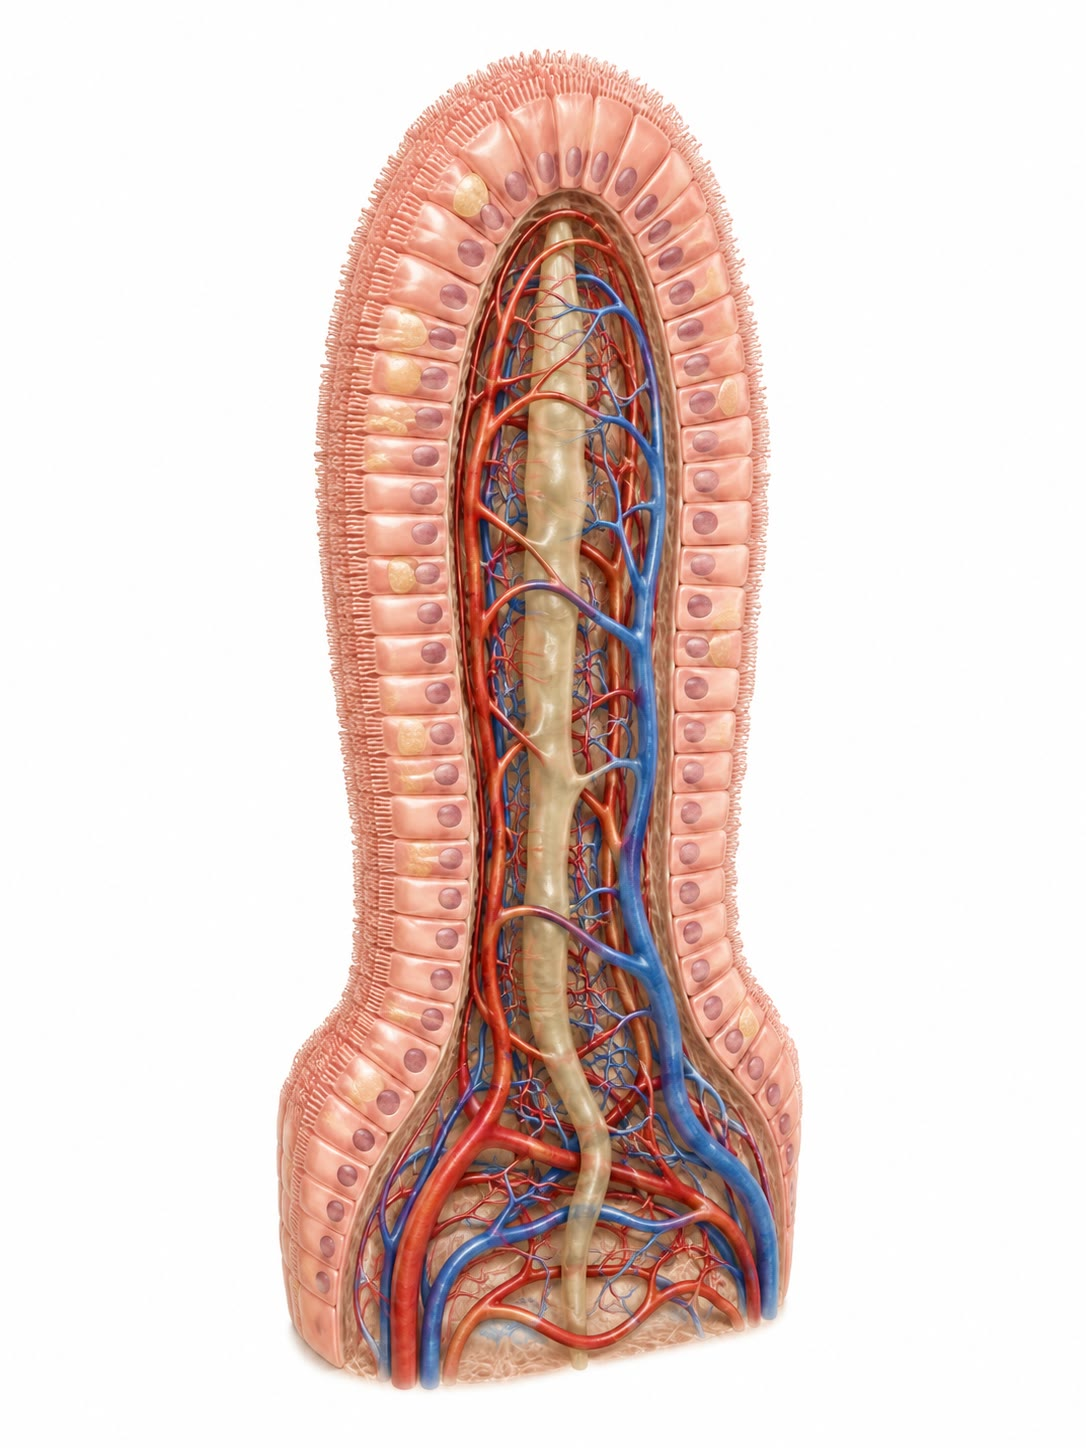
\includegraphics[width=0.36\linewidth]{images/book3/ai/fig-villus-cutaway.jpg}};
  \begin{scope}[x={(img.south east)}, y={(img.north west)},
      every node/.style={font=\small}]
    \draw[omDef, thick] (0.25,0.80) -- (-0.05,0.88) node[left, align=right] {单层 \\ 肠上皮细胞};
    \draw[omDef, thick] (0.50,0.55) -- (1.05,0.62) node[right, align=left] {中央乳糜管：\\ 脂肪入淋巴};
    \draw[omDef, thick] (0.70,0.40) -- (1.05,0.36) node[right, align=left] {毛细血管：糖与 \\ 氨基酸入门静脉};
    \draw[omDef, thick] (0.30,0.15) -- (-0.05,0.10) node[left, align=right] {隐窝：细胞 \\ 在此更新};
  \end{scope}
\end{tikzpicture}

{\small 剖开的\omterm{def:b1:digestion-absorption:surface}{绒毛}：一层\omterm{def:b1:digestion-absorption:nutrition}{吸收}\omterm{def:b1:cell-unit-of-life:cell}{细胞}覆盖在
承载淋巴管与毛细血管网的核心之上。每个被\omterm{def:b1:digestion-absorption:nutrition}{吸收}的
分子需穿过两层膜和几微米厚的\omterm{def:b1:body-plans-tissues:tissue}{组织}。}
\end{omfigure}

\begin{proposition}[吸收途径]\label{prop:b1:digestion-absorption:routes}
\index{乳糜微粒}
\emph{\omterm{def:b1:carbohydrates:monosaccharide}{糖类}}：葡萄糖与半乳糖经
钠–葡萄糖\omterm{prop:b1:membranes-transport:secondary}{同向转运体}（见\cref{ch:b1:membranes-transport}）转运，果糖
经载体转运，三者均由基底侧的载体
运入血液。\emph{\omterm{def:b1:proteins:aminoacid}{氨基酸}}经数种钠偶联\omterm{prop:b1:membranes-transport:secondary}{同向转运体}
进入，小肽经一种质子偶联转运体运入，并在\omterm{def:b1:cell-unit-of-life:cell}{细胞}内被切割。
\emph{\omterm{def:b1:lipids:triglyceride}{脂肪}}：\omterm{def:b1:lipids:fattyacid}{脂肪酸}与单甘油酯离开胶束，
经顶端膜扩散进入\omterm{def:b1:cell-unit-of-life:cell}{细胞}；在\omterm{def:b1:cell-unit-of-life:cell}{细胞}内，它们
重新酯化为\omterm{def:b1:lipids:triglyceride}{甘油三酯}，并包裹\omterm{def:b1:proteins:peptide}{蛋白质}，形成
直径约 1 微米的\emph{乳糜微粒}，经胞吐进入
乳糜管。\omterm{def:b1:mammal-organization:compartments}{淋巴液}仅在颈部汇入血液，\omterm{def:b1:lipids:triglyceride}{脂肪}由此
绕过肝脏。\emph{水}通过\omterm{def:b1:membranes-transport:osmosis}{渗透作用}随溶质移动：
每天有 \qty{9}{L} 进入肠道（其中饮入 2 升，7 升
由唾液、胃液、胆汁及胰液、肠液分泌），除 0.1 升外
全部被重\omterm{def:b1:digestion-absorption:nutrition}{吸收}，大部分在小肠，
少部分在结肠。\emph{维生素}、\emph{铁}与\emph{钙}
各有其载体；维生素 B$_{12}$ 需要胃中的一种
\omterm{def:b1:proteins:peptide}{蛋白质}才能被\omterm{def:b1:digestion-absorption:nutrition}{吸收}。
\end{proposition}

\begin{omfigure}
\begin{tikzpicture}[font=\footnotesize, >=Stealth, line cap=round]
  % lumen | enterocyte | blood/lymph
  \fill[omDef!8] (0,0) rectangle (4.2,5.2); \node[anchor=north, font=\small] at (2.1,5.1) {肠腔};
  \fill[omProp!10] (4.5,0) rectangle (8.7,5.2); \node[anchor=north, font=\small] at (6.6,5.1) {肠上皮细胞};
  \fill[omThm!8] (9.0,0) rectangle (12.6,5.2); \node[anchor=north, font=\small] at (10.8,5.1) {血液或淋巴};
  \draw[very thick, omDef!60!black] (4.35,0) -- (4.35,5.2); \draw[very thick, omDef!60!black] (8.85,0) -- (8.85,5.2);
  \node[font=\scriptsize, rotate=90, anchor=south] at (4.2,2.6) {顶端（刷状缘）};
  \node[font=\scriptsize, rotate=90, anchor=north] at (9.0,2.6) {基底侧};
  % sugars
  \node[anchor=east] at (3.75,4.2) {葡萄糖、半乳糖};
  \draw[->, very thick, omExo!70!black] (4.1,4.2) -- (4.7,4.2) node[right, font=\scriptsize] {$\mathrm{Na^+}$ 同向转运};
  \draw[->, very thick, omProp!80!black] (8.5,4.2) -- (9.3,4.2) node[right, font=\scriptsize] {载体 $\to$ 门静脉};
  % amino acids
  \node[anchor=east] at (3.75,3.2) {氨基酸、小肽};
  \draw[->, very thick, omExo!70!black] (4.1,3.2) -- (4.7,3.2) node[right, font=\scriptsize] {$\mathrm{Na^+}$ / $\mathrm{H^+}$ 同向转运};
  \draw[->, very thick, omProp!80!black] (8.5,3.2) -- (9.3,3.2) node[right, font=\scriptsize] {载体 $\to$ 门静脉};
  % fats
  \node[anchor=east, align=right] at (3.75,2.0) {脂肪酸、单甘油酯 \\ （位于胶束中）};
  \draw[->, very thick, omDef!70!black] (4.1,2.0) -- (4.7,2.0) node[right, font=\scriptsize] {扩散};
  \node[font=\scriptsize, align=center] at (6.7,1.5) {重新酯化，\\ 包装成乳糜微粒};
  \draw[->, very thick, omProp!80!black] (8.5,2.0) -- (9.3,2.0) node[right, font=\scriptsize] {胞吐 $\to$ 乳糜管};
  % water
  \node[anchor=east] at (3.75,0.7) {水（每天 \qty{9}{L}）};
  \draw[->, very thick, gray] (4.1,0.7) -- (9.3,0.7) node[right, font=\scriptsize] {渗透作用，随溶质移动};
\end{tikzpicture}

{\small 穿过\omterm{def:b1:digestion-absorption:surface}{肠上皮细胞}的四条途径。\omterm{def:b1:carbohydrates:monosaccharide}{糖类}与\omterm{def:b1:proteins:aminoacid}{氨基酸}
经钠偶联转运进入，并经载体转运至
血液；\omterm{def:b1:lipids:triglyceride}{脂肪}自胶束扩散进入，重新合成后以
乳糜微粒形式进入淋巴；水随之移动。}
\end{omfigure}

\begin{method}[解读吸收实验]\label{met:b1:digestion-absorption:everted}
\begin{enumerate}
  \item 将一段肠管翻转过来（制成\emph{外翻囊}），
        内充生理盐水，再将其浸入含该物质的溶液中：
        出现在囊内的物质，已穿过\omterm{def:b1:body-plans-tissues:epithelium}{上皮}，
        由原来的肠腔转入。
  \item 测定转运与浓度的关系：呈饱和性，
        且被低温或 \omterm{def:b1:water-small-molecules:atp}{ATP} 合成\omterm{def:b1:enzymes:inhibitors}{抑制剂}所阻断——为主动转运或载体介导；
        呈线性且不受影响——为扩散。
  \item 从浴液中去除钠：若葡萄糖或\omterm{def:b1:proteins:aminoacid}{氨基酸}的转运随之消失，
        则其为钠偶联转运。加入\omterm{def:b1:enzymes:inhibitors}{竞争性}\omterm{def:b1:carbohydrates:monosaccharide}{糖类}：
        若转运下降，则二者共用同一载体。
  \item 比较各段肠道：大多数\omterm{def:b1:carbohydrates:monosaccharide}{糖类}和\omterm{def:b1:proteins:aminoacid}{氨基酸}在空肠中透过，
        胆盐与维生素 B$_{12}$仅在回肠中透过，
        水和盐则在各段均可透过。
\end{enumerate}
\end{method}

\begin{example}[水量收支]\label{ex:b1:digestion-absorption:water}
每天进入人体肠道的九升液体中，小肠\omterm{def:b1:digestion-absorption:nutrition}{吸收}八升，
结肠再\omterm{def:b1:digestion-absorption:nutrition}{吸收}一升，仅 \qty{0.1}{L} 随粪便排出。
小肠对葡萄糖的钠偶联摄取会带动水分随之移动——
这就是为何霍乱患儿口服葡萄糖与
盐的溶液可以补充水分：毒素使隐窝转为分泌型，
\omterm{prop:b1:membranes-transport:secondary}{同向转运体}未受影响，其\omterm{def:b1:digestion-absorption:nutrition}{吸收}水分的速度
快于毒素使水分流失的速度，
（见\cref{ch:b1:membranes-transport}）。
\end{example}

\section{以草为食}

\begin{proposition}[纤维素的共生消化]\label{prop:b1:digestion-absorption:cellulose}
\index{瘤胃}\index{反刍动物}\index{后肠发酵}
没有哺乳动物能合成\omterm{def:b1:carbohydrates:polysaccharide}{纤维素}酶。植食性动物依靠饲养
能分解\omterm{def:b1:carbohydrates:polysaccharide}{纤维素}的细菌、原生生物和真菌来\omterm{def:b1:digestion-absorption:nutrition}{消化}\omterm{def:b1:carbohydrates:polysaccharide}{纤维素}，它们位于\omterm{def:b1:respiration-fermentation:fermentation}{发酵}室中，
微生物断裂 $\beta(1{\to}4)$ 键（见\cref{ch:b1:carbohydrates}）
并在无氧条件下将\omterm{def:b1:carbohydrates:monosaccharide}{糖类}\omterm{def:b1:respiration-fermentation:fermentation}{发酵}为\emph{挥发性\omterm{def:b1:lipids:fattyacid}{脂肪酸}}
——乙酸、丙酸、丁酸——以及二氧化碳和甲烷。
宿主\omterm{def:b1:digestion-absorption:nutrition}{吸收}这些酸并以之为生。\emph{反刍动物}（牛、
绵羊、鹿）将\omterm{def:b1:respiration-fermentation:fermentation}{发酵}室置于真正的胃\emph{之前}：
即\emph{瘤胃}，牛体内容量达一百升的大槽，食物在其中
\omterm{def:b1:respiration-fermentation:fermentation}{发酵}一两天，经反刍和再次咀嚼，并由此
使微生物本身进入皱胃和肠道，
作为动物主要的\omterm{def:b1:proteins:peptide}{蛋白质}来源而被\omterm{def:b1:digestion-absorption:nutrition}{消化}。\emph{后肠
\omterm{def:b1:respiration-fermentation:fermentation}{发酵}动物}（马、兔子、大象）把\omterm{def:b1:respiration-fermentation:fermentation}{发酵}室放在小肠\emph{之后}，
位于增大的盲肠和结肠中：它们先自行\omterm{def:b1:digestion-absorption:nutrition}{消化}\omterm{def:b1:carbohydrates:polysaccharide}{淀粉}和\omterm{def:b1:proteins:peptide}{蛋白质}，
之后再\omterm{def:b1:respiration-fermentation:fermentation}{发酵}纤维，并
使微生物蛋白随粪便流失——除非像兔子那样，
它们食用柔软的夜间粪便，使其再经过一次
\omterm{prop:b1:digestion-absorption:tract}{消化道}（\emph{盲肠营养}）。
\end{proposition}

\begin{omfigure}
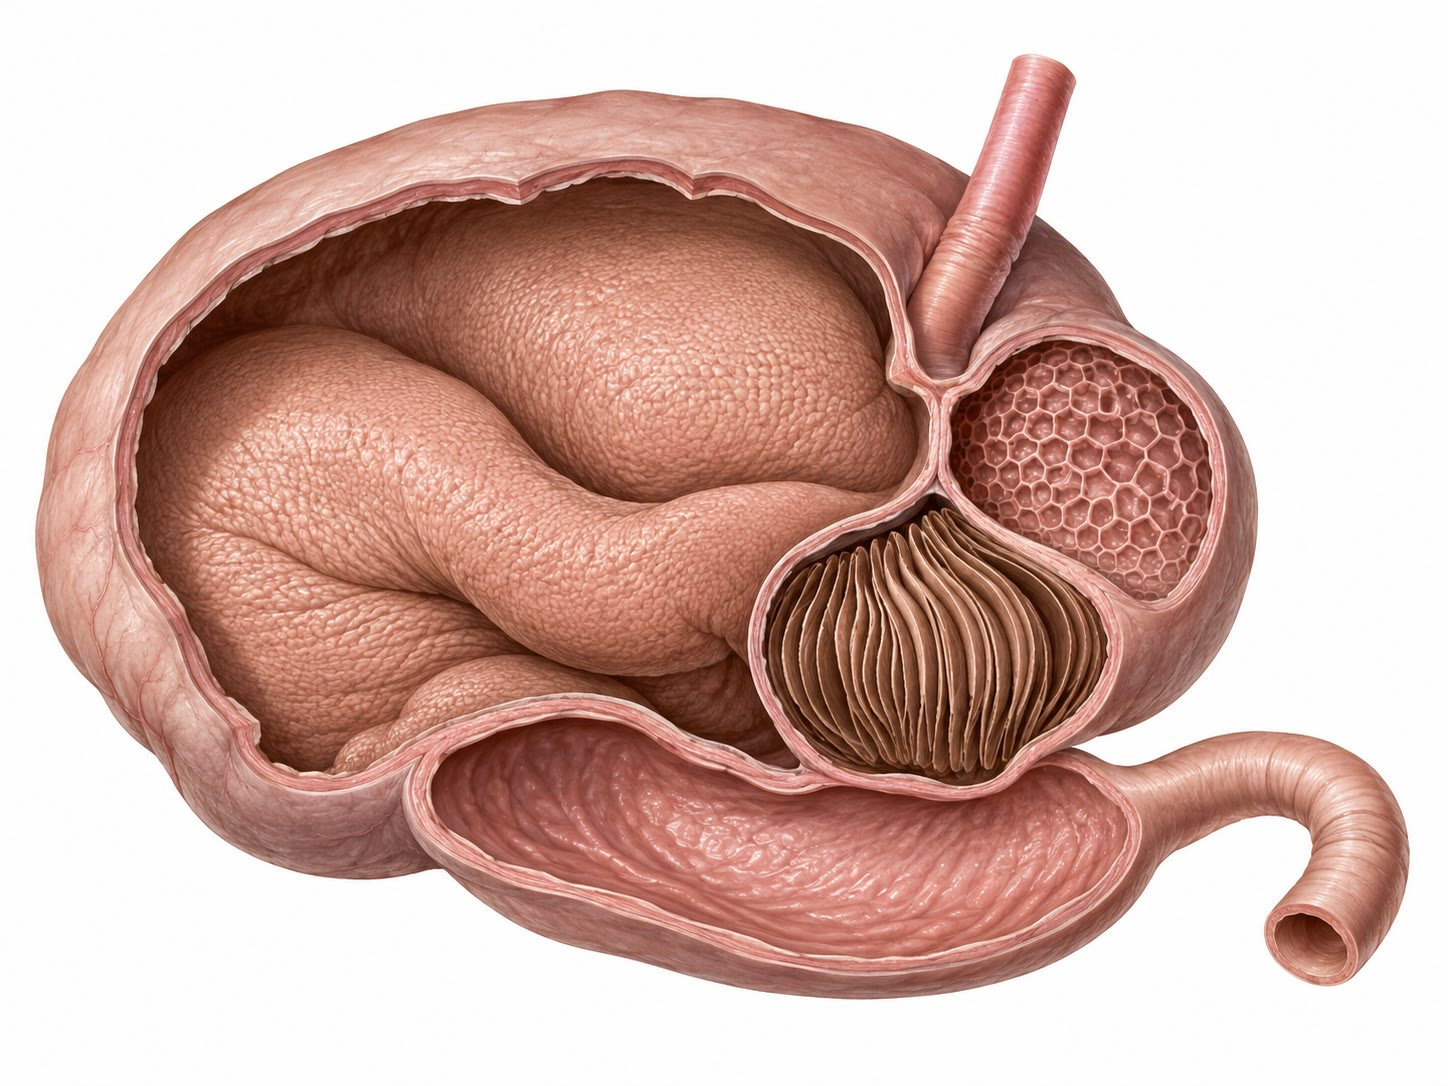
\includegraphics[width=0.56\linewidth]{images/book3/ai/b3-22-ruminant-stomach.jpg}

{\small 牛的四室胃：巨大的瘤胃和
网胃是微生物\omterm{def:b1:respiration-fermentation:fermentation}{发酵}的场所，瓣胃的叶片可\omterm{def:b1:digestion-absorption:nutrition}{吸收}
水分，皱胃是真正的酸性胃，
其中微生物被\omterm{def:b1:digestion-absorption:nutrition}{消化}。}
\end{omfigure}

\begin{example}[吃草地的两种方式]\label{ex:b1:digestion-absorption:cowhorse}
牛\omterm{def:b1:respiration-fermentation:fermentation}{发酵}约三分之二的纤维，其能量的百分之六十以乙酸和丙酸的形式获得，
——由此其肝脏须合成所需的每一克葡萄糖，
因为几乎没有葡萄糖能到达肠道；
其瘤胃还能将由血液回流至唾液中的尿素所含的氮
转化为微生物蛋白，因而牛能以\omterm{def:b1:proteins:peptide}{蛋白质}含量
比其他任何哺乳动物所能忍受的都更低的干草为食。
马\omterm{def:b1:respiration-fermentation:fermentation}{发酵}的纤维不足一半，但自行\omterm{def:b1:digestion-absorption:nutrition}{消化}草的\omterm{def:b1:carbohydrates:polysaccharide}{淀粉}和\omterm{def:b1:proteins:peptide}{蛋白质}，
\omterm{def:b1:digestion-absorption:nutrition}{吸收}葡萄糖，食物通过\omterm{prop:b1:digestion-absorption:tract}{消化道}仅需一天半，而非
三天：它从每千克食物中获取的能量较少，故需进食更多。
贫瘠草场上牛占优，马则在必须奔跑时占优。
\end{example}

\begin{remark}[肠道的长度]\label{rem:b1:digestion-absorption:length}
肉食性动物的肠道长度为其体长的四倍，植食性动物则为
十至二十倍：食物越差，肠道越长，\omterm{def:b1:digestion-absorption:nutrition}{消化}腔室也越大。
以藻类为食的蝌蚪有一段盘曲的长肠，
在变态时，青蛙转为捕食昆虫，肠道便骤然变短；
同一规律在一个动物的一生中得以体现。
\end{remark}

\section{练习}

\begin{exercise}[$\star$]\label{exo:b1:digestion-absorption:1}
列出\omterm{prop:b1:digestion-absorption:tract}{消化道}各部分，并说明每一部分的主要\omterm{def:b1:digestion-absorption:nutrition}{消化}事件。
\end{exercise}

\begin{exercise}[$\star$]\label{exo:b1:digestion-absorption:2}
哪些酶参与\omterm{def:b1:proteins:peptide}{蛋白质}的\omterm{def:b1:digestion-absorption:nutrition}{消化}？它们分别在何处发挥作用，
各自在何种 \omterm{def:b1:water-small-molecules:ph}{pH} 下起作用？为何它们以酶原形式合成？
\end{exercise}

\begin{exercise}[$\star$]\label{exo:b1:digestion-absorption:3}
根据\omterm{def:b1:digestion-absorption:nutrition}{吸收}示意图，说出葡萄糖、一种\omterm{def:b1:proteins:aminoacid}{氨基酸}和一种\omterm{def:b1:lipids:fattyacid}{脂肪酸}
穿过\omterm{def:b1:digestion-absorption:surface}{肠上皮细胞}所经的途径，并指出各自最终进入何处。
\end{exercise}

\begin{exercise}[$\star$]\label{exo:b1:digestion-absorption:4}
胆汁有何作用？在\omterm{def:b1:lipids:triglyceride}{脂肪}酶存在的情况下，
缺乏胆汁为何仍会导致\omterm{def:b1:lipids:triglyceride}{脂肪}\omterm{def:b1:digestion-absorption:nutrition}{消化}失败？
\end{exercise}

\begin{exercise}[$\star\star$]\label{exo:b1:digestion-absorption:5}
一餐中含 \qty{100}{g} \omterm{def:b1:carbohydrates:polysaccharide}{淀粉}，三小时内被\omterm{def:b1:digestion-absorption:nutrition}{消化}为葡萄糖。
计算被水解的\omterm{def:b1:carbohydrates:glycosidic}{糖苷键}的摩尔数、
消耗的水量，以及葡萄糖\omterm{def:b1:digestion-absorption:nutrition}{吸收}的平均速率
（以毫摩尔每分钟计）。
\end{exercise}

\begin{exercise}[$\star\star$]\label{exo:b1:digestion-absorption:6}
结合本章所述激素，说明酸性食糜和\omterm{def:b1:lipids:triglyceride}{脂肪}从胃进入十二指肠后
最初数分钟内十二指肠中发生的变化，
以及胃随后为何减慢排空。
\end{exercise}

\begin{exercise}[$\star\star$]\label{exo:b1:digestion-absorption:7}
一个外翻肠囊从 \qty{5}{mmol/L} 的浴液中转运葡萄糖，
直至囊内达到 \qty{40}{mmol/L}；若将浴液中的钠换为钾，
则囊内停在 \qty{5}{mmol/L}。解释这两种
结果。
\end{exercise}

\begin{exercise}[$\star\star$]\label{exo:b1:digestion-absorption:8}
为何\omterm{def:b1:lipids:triglyceride}{脂肪}经淋巴而不经门静脉进入血液，
若乳糜微粒直接进入门静脉血液，
会出现什么情况？
\end{exercise}

\begin{exercise}[$\star\star$]\label{exo:b1:digestion-absorption:9}
一头牛每天分泌 \qty{100}{L} 唾液。解释这种唾液
在反刍动物中的三项作用，其中一项与氮有关。
\end{exercise}

\begin{exercise}[$\star\star\star$]\label{exo:b1:digestion-absorption:10}
某患者的胰腺功能衰竭。预测各类
营养物质的去向、粪便的外观，以及哪些食物
仍能被残存的酶\omterm{def:b1:digestion-absorption:nutrition}{消化}。
\end{exercise}

\begin{exercise}[$\star\star\star$]\label{exo:b1:digestion-absorption:11}
阻止兔子食用其夜间粪便后，它在对照兔子
生长良好的日粮上仍然减重。解释它损失的是什么，为何牛
不需要这种习性，又为何马同样无法
弥补这一损失。
\end{exercise}

\begin{exercise}[$\star\star\star$]\label{exo:b1:digestion-absorption:12}
“牛是长着腿的\omterm{def:b1:respiration-fermentation:fermentation}{发酵}罐。”请用一段文字讨论：微生物为牛提供了什么
（能量、\omterm{def:b1:proteins:peptide}{蛋白质}、维生素），牛为微生物提供了什么，
以及这一设计在何处失效（甲烷、葡萄糖、速度）。
\end{exercise}

\section{问题：牛与马}

\begin{problem}[{周末问题——十千克干草经瘤胃与盲肠：
纤维被发酵，酸被吸收，微生物蛋白有所增减，
甲烷被排出，以牛能量中来自挥发性脂肪酸的
比例收尾}]
\label{pb:b1:digestion-absorption:1}
牛与马每天各采食 \qty{10}{kg} 干草干物质，
按质量计，含 \qty{50}{\%} \omterm{def:b1:carbohydrates:polysaccharide}{纤维素}和半\omterm{def:b1:carbohydrates:polysaccharide}{纤维素}（纤维），
\qty{20}{\%} \omterm{def:b1:carbohydrates:polysaccharide}{淀粉}和\omterm{def:b1:carbohydrates:monosaccharide}{糖类}，\qty{15}{\%} \omterm{def:b1:proteins:peptide}{蛋白质}和 \qty{15}{\%}
难\omterm{def:b1:digestion-absorption:nutrition}{消化}的木质素和灰分。能量：碳水化合物和\omterm{def:b1:proteins:peptide}{蛋白质}
各为 \qty{17.5}{kJ/g}。\omterm{def:b1:respiration-fermentation:fermentation}{发酵} \qty{1}{g} 碳水化合物可产生
挥发性\omterm{def:b1:lipids:fattyacid}{脂肪酸}，其所含能量占 \qty{75}{\%}，甲烷占
\qty{8}{\%}，其余为热量和微生物生长；此外还产生
\qty{0.15}{g} 微生物蛋白。瘤胃\omterm{def:b1:respiration-fermentation:fermentation}{发酵}
\qty{70}{\%} 的纤维以及全部\omterm{def:b1:carbohydrates:polysaccharide}{淀粉}和\omterm{def:b1:carbohydrates:monosaccharide}{糖类}；马的
后肠\omterm{def:b1:respiration-fermentation:fermentation}{发酵} \qty{45}{\%} 的纤维，而其小肠
\omterm{def:b1:digestion-absorption:nutrition}{消化} \qty{90}{\%} 的\omterm{def:b1:carbohydrates:polysaccharide}{淀粉}和 \qty{70}{\%} 的\omterm{def:b1:proteins:peptide}{蛋白质}，
然后纤维才进入后肠。两种动物每天都需要 \qty{110}{MJ}
的可代谢能。

\medskip
\noindent\textbf{第一部分——牛的瘤胃。}
\begin{enumerate}
  \item 计算每日所食纤维、\omterm{def:b1:carbohydrates:polysaccharide}{淀粉}和\omterm{def:b1:carbohydrates:monosaccharide}{糖类}以及
        \omterm{def:b1:proteins:peptide}{蛋白质}的质量。
  \item 计算在瘤胃中\omterm{def:b1:respiration-fermentation:fermentation}{发酵}的碳水化合物的质量。
  \item 计算该碳水化合物的能量，以及
        以挥发性\omterm{def:b1:lipids:fattyacid}{脂肪酸}形式回收的能量。
  \item 计算以甲烷形式损失的能量，以及甲烷的质量
        （\qty{55}{kJ/g}）及其体积（\qty{1.4}{L/g}）。
  \item 计算产生的微生物蛋白的质量。
  \item 解释为什么牛自身的\omterm{def:b1:proteins:peptide}{蛋白质}来源主要是
        微生物，以及它们在何处被\omterm{def:b1:digestion-absorption:nutrition}{消化}。
  \item 计算离开瘤胃而未被\omterm{def:b1:respiration-fermentation:fermentation}{发酵}的纤维比例，
        及其去向。
\end{enumerate}

\medskip
\noindent\textbf{第二部分——牛的能量平衡。}
牛还\omterm{def:b1:digestion-absorption:nutrition}{消化} \qty{60}{\%} 逃逸瘤胃的膳食\omterm{def:b1:proteins:peptide}{蛋白质}
（所食\omterm{def:b1:proteins:peptide}{蛋白质}中有 \qty{40}{\%} 逃逸），以及全部
微生物蛋白，能量按 \qty{17.5}{kJ/g} 计。
\begin{enumerate}[resume]
  \item 计算牛从\omterm{def:b1:proteins:peptide}{蛋白质}（膳食逃逸部分
        加微生物蛋白）中获得的能量。
  \item 计算牛的可代谢能总量：挥发性\omterm{def:b1:lipids:fattyacid}{脂肪
        酸}加\omterm{def:b1:proteins:peptide}{蛋白质}。
  \item 计算该能量中由挥发性\omterm{def:b1:lipids:fattyacid}{脂肪
        酸}提供的比例。
  \item 牛能否满足其 \qty{110}{MJ} 的需要？若不能，
        她将如何应对？
  \item 牛几乎不\omterm{def:b1:digestion-absorption:nutrition}{吸收}葡萄糖。写出其肝脏
        由哪种酸合成葡萄糖，以及该过程的名称。
\end{enumerate}

\medskip
\noindent\textbf{第三部分——马的后肠。}
\begin{enumerate}[resume]
  \item 计算马在小肠中\omterm{def:b1:digestion-absorption:nutrition}{消化}\omterm{def:b1:carbohydrates:polysaccharide}{淀粉}所获得的能量
        （以葡萄糖形式\omterm{def:b1:digestion-absorption:nutrition}{吸收}，\qty{17.5}{kJ/g}）。
  \item 计算小肠中\omterm{def:b1:digestion-absorption:nutrition}{消化}的膳食\omterm{def:b1:proteins:peptide}{蛋白质}
        提供的能量。
  \item 计算后肠中\omterm{def:b1:respiration-fermentation:fermentation}{发酵}的纤维量，以及
        以挥发性\omterm{def:b1:lipids:fattyacid}{脂肪酸}形式回收的能量。
  \item 计算后肠产生的微生物\omterm{def:b1:proteins:peptide}{蛋白质}。它
        去向如何？
  \item 计算马的可代谢能总量，以及
        由挥发性\omterm{def:b1:lipids:fattyacid}{脂肪酸}提供的比例。
  \item 马能否满足其 \qty{110}{MJ} 的需要？它需要
        采食多少干草，又是如何做到的？
\end{enumerate}

\medskip
\noindent\textbf{第四部分——比较两种设计。}
\begin{enumerate}[resume]
  \item 计算每种动物每千克干草
        干物质所提取的能量。
  \item 牛的甲烷占\omterm{def:b1:respiration-fermentation:fermentation}{发酵}能量的 \qty{8}{\%}，
        计算其占牛总摄入能量的比例，以及
        一群一百头牛一年排放的甲烷质量。
  \item 牛的食物在\omterm{prop:b1:digestion-absorption:tract}{消化道}中停留 \qty{70}{h}，马的
        为 \qty{36}{h}。计算采食量恒定时，两者
        任一时刻\omterm{prop:b1:digestion-absorption:tract}{消化道}内所含干物质的质量。
  \item 兔子在盲肠中\omterm{def:b1:respiration-fermentation:fermentation}{发酵}纤维，然后食用其
        盲肠粪便。问题 16 中的微生物蛋白，
        马若同样这样做，能回收其中多大比例？为何
        没有马这样做？
  \item 解释为何牛能以秸秆加尿素为食，
        其中含 \qty{4}{\%} \omterm{def:b1:proteins:peptide}{蛋白质}，而马不能。
  \item 冲刺中的马燃烧自身\omterm{def:b1:carbohydrates:polysaccharide}{糖原}中的葡萄糖；牛
        不能冲刺。请结合两种设计加以分析。
  \item 给出结果：牛的可代谢能中来自挥发性\omterm{def:b1:lipids:fattyacid}{脂肪酸}的比例，
        马的相应比例，
        以及两者每千克干草所提取的能量。
\end{enumerate}
\end{problem}
